\documentclass[11pt, a4paper]{article}
\usepackage{pdfpages}
\usepackage{parallel}
\usepackage[T2A]{fontenc}
\usepackage{ucs}
\usepackage[utf8x]{inputenc}
\usepackage[polish,english,russian]{babel}
\usepackage{hyperref}
\usepackage{rotating}
\usepackage[inner=2cm,top=1.8cm,outer=2cm,bottom=2.3cm,nohead]{geometry}
\usepackage{listings}
\usepackage{graphicx}
\usepackage{wrapfig}
\usepackage{longtable}
\usepackage{indentfirst}
\usepackage{array}
\usepackage{tikzsymbols}
\usepackage{soul}
\usepackage[ruled,vlined]{algorithm2e}
%\counterwithout{figure}{section} 

\usepackage{url}
\makeatletter
\g@addto@macro{\UrlBreaks}{\UrlOrds}
\makeatother

\newcolumntype{P}[1]{>{\raggedright\arraybackslash}p{#1}}
\frenchspacing
\usepackage{fixltx2e} %text sub- and superscripts
\usepackage{icomma} % коскі ў матэматычным рэжыме
\PreloadUnicodePage{4}

\newcommand{\longpage}{\enlargethispage{\baselineskip}}
\newcommand{\shortpage}{\enlargethispage{-\baselineskip}}

\def\switchlang#1{\expandafter\csname switchlang#1\endcsname}
\def\switchlangbe{
\let\saverefname=\refname%
\def\refname{Літаратура}%
\def\figurename{Іл.}%
}
\def\switchlangen{
\let\saverefname=\refname%
\def\refname{References}%
\def\figurename{Fig.}%
}
\def\switchlangru{
\let\saverefname=\refname%
\let\savefigurename=\figurename%
\def\refname{Литература}%
\def\figurename{Рис.}%
}

\hyphenation{admi-ni-stra-tive}
\hyphenation{ex-pe-ri-ence}
\hyphenation{fle-xi-bi-li-ty}
\hyphenation{Py-thon}
\hyphenation{ma-the-ma-ti-cal}
\hyphenation{re-ported}
\hyphenation{imp-le-menta-tions}
\hyphenation{pro-vides}
\hyphenation{en-gi-neering}
\hyphenation{com-pa-ti-bi-li-ty}
\hyphenation{im-pos-sible}
\hyphenation{desk-top}
\hyphenation{elec-tro-nic}
\hyphenation{com-pa-ny}
\hyphenation{de-ve-lop-ment}
\hyphenation{de-ve-loping}
\hyphenation{de-ve-lop}
\hyphenation{da-ta-ba-se}
\hyphenation{plat-forms}
\hyphenation{or-ga-ni-za-tion}
\hyphenation{pro-gramming}
\hyphenation{in-stru-ments}
\hyphenation{Li-nux}
\hyphenation{sour-ce}
\hyphenation{en-vi-ron-ment}
\hyphenation{Te-le-pathy}
\hyphenation{Li-nux-ov-ka}
\hyphenation{Open-BSD}
\hyphenation{Free-BSD}
\hyphenation{men-ti-on-ed}
\hyphenation{app-li-ca-tion}

\def\progref!#1!{\texttt{#1}}
\renewcommand{\arraystretch}{2} %Іначай формулы ў матрыцы зліпаюцца з лініямі
\usepackage{array}

\def\interview #1 (#2), #3, #4, #5\par{

\section[#1, #3, #4]{#1 -- #3, #4}
\def\qname{LVEE}
\def\aname{#1}
\def\q ##1\par{{\noindent \bf \qname: ##1 }\par}
\def\a{{\noindent \bf \aname: } \def\qname{L}\def\aname{#2}}
}

\def\interview* #1 (#2), #3, #4, #5\par{

\section*{#1\\{\small\rm #3, #4. #5}}
\ifx\ParallelWhichBox\undefined%
    \addcontentsline{toc}{section}{#1, #3, #4}%
\else%
\ifnum\ParallelWhichBox=0%
    \addcontentsline{toc}{section}{#1, #3, #4}%
\fi\fi%

\def\qname{LVEE}
\def\aname{#1}
\def\q ##1\par{{\noindent \bf \qname: ##1 }\par}
\def\a{{\noindent \bf \aname: } \def\qname{L}\def\aname{#2}}
}

\newcommand{\interviewfooter}[1]{
\vskip 1em
\noindent \textit{#1}
}

\switchlang{en}
\begin{document}

\title{1983 "--- Apple Lisa mouse}
\date{}
\maketitle
\selectlanguage{english}
The Apple Lisa mouse was released in 1983 \cite{mouses} and is considered one of the first commercially available computer mice (figure \ref{fig:AppleLisaPic}).

\begin{figure}[h]
   \centering
    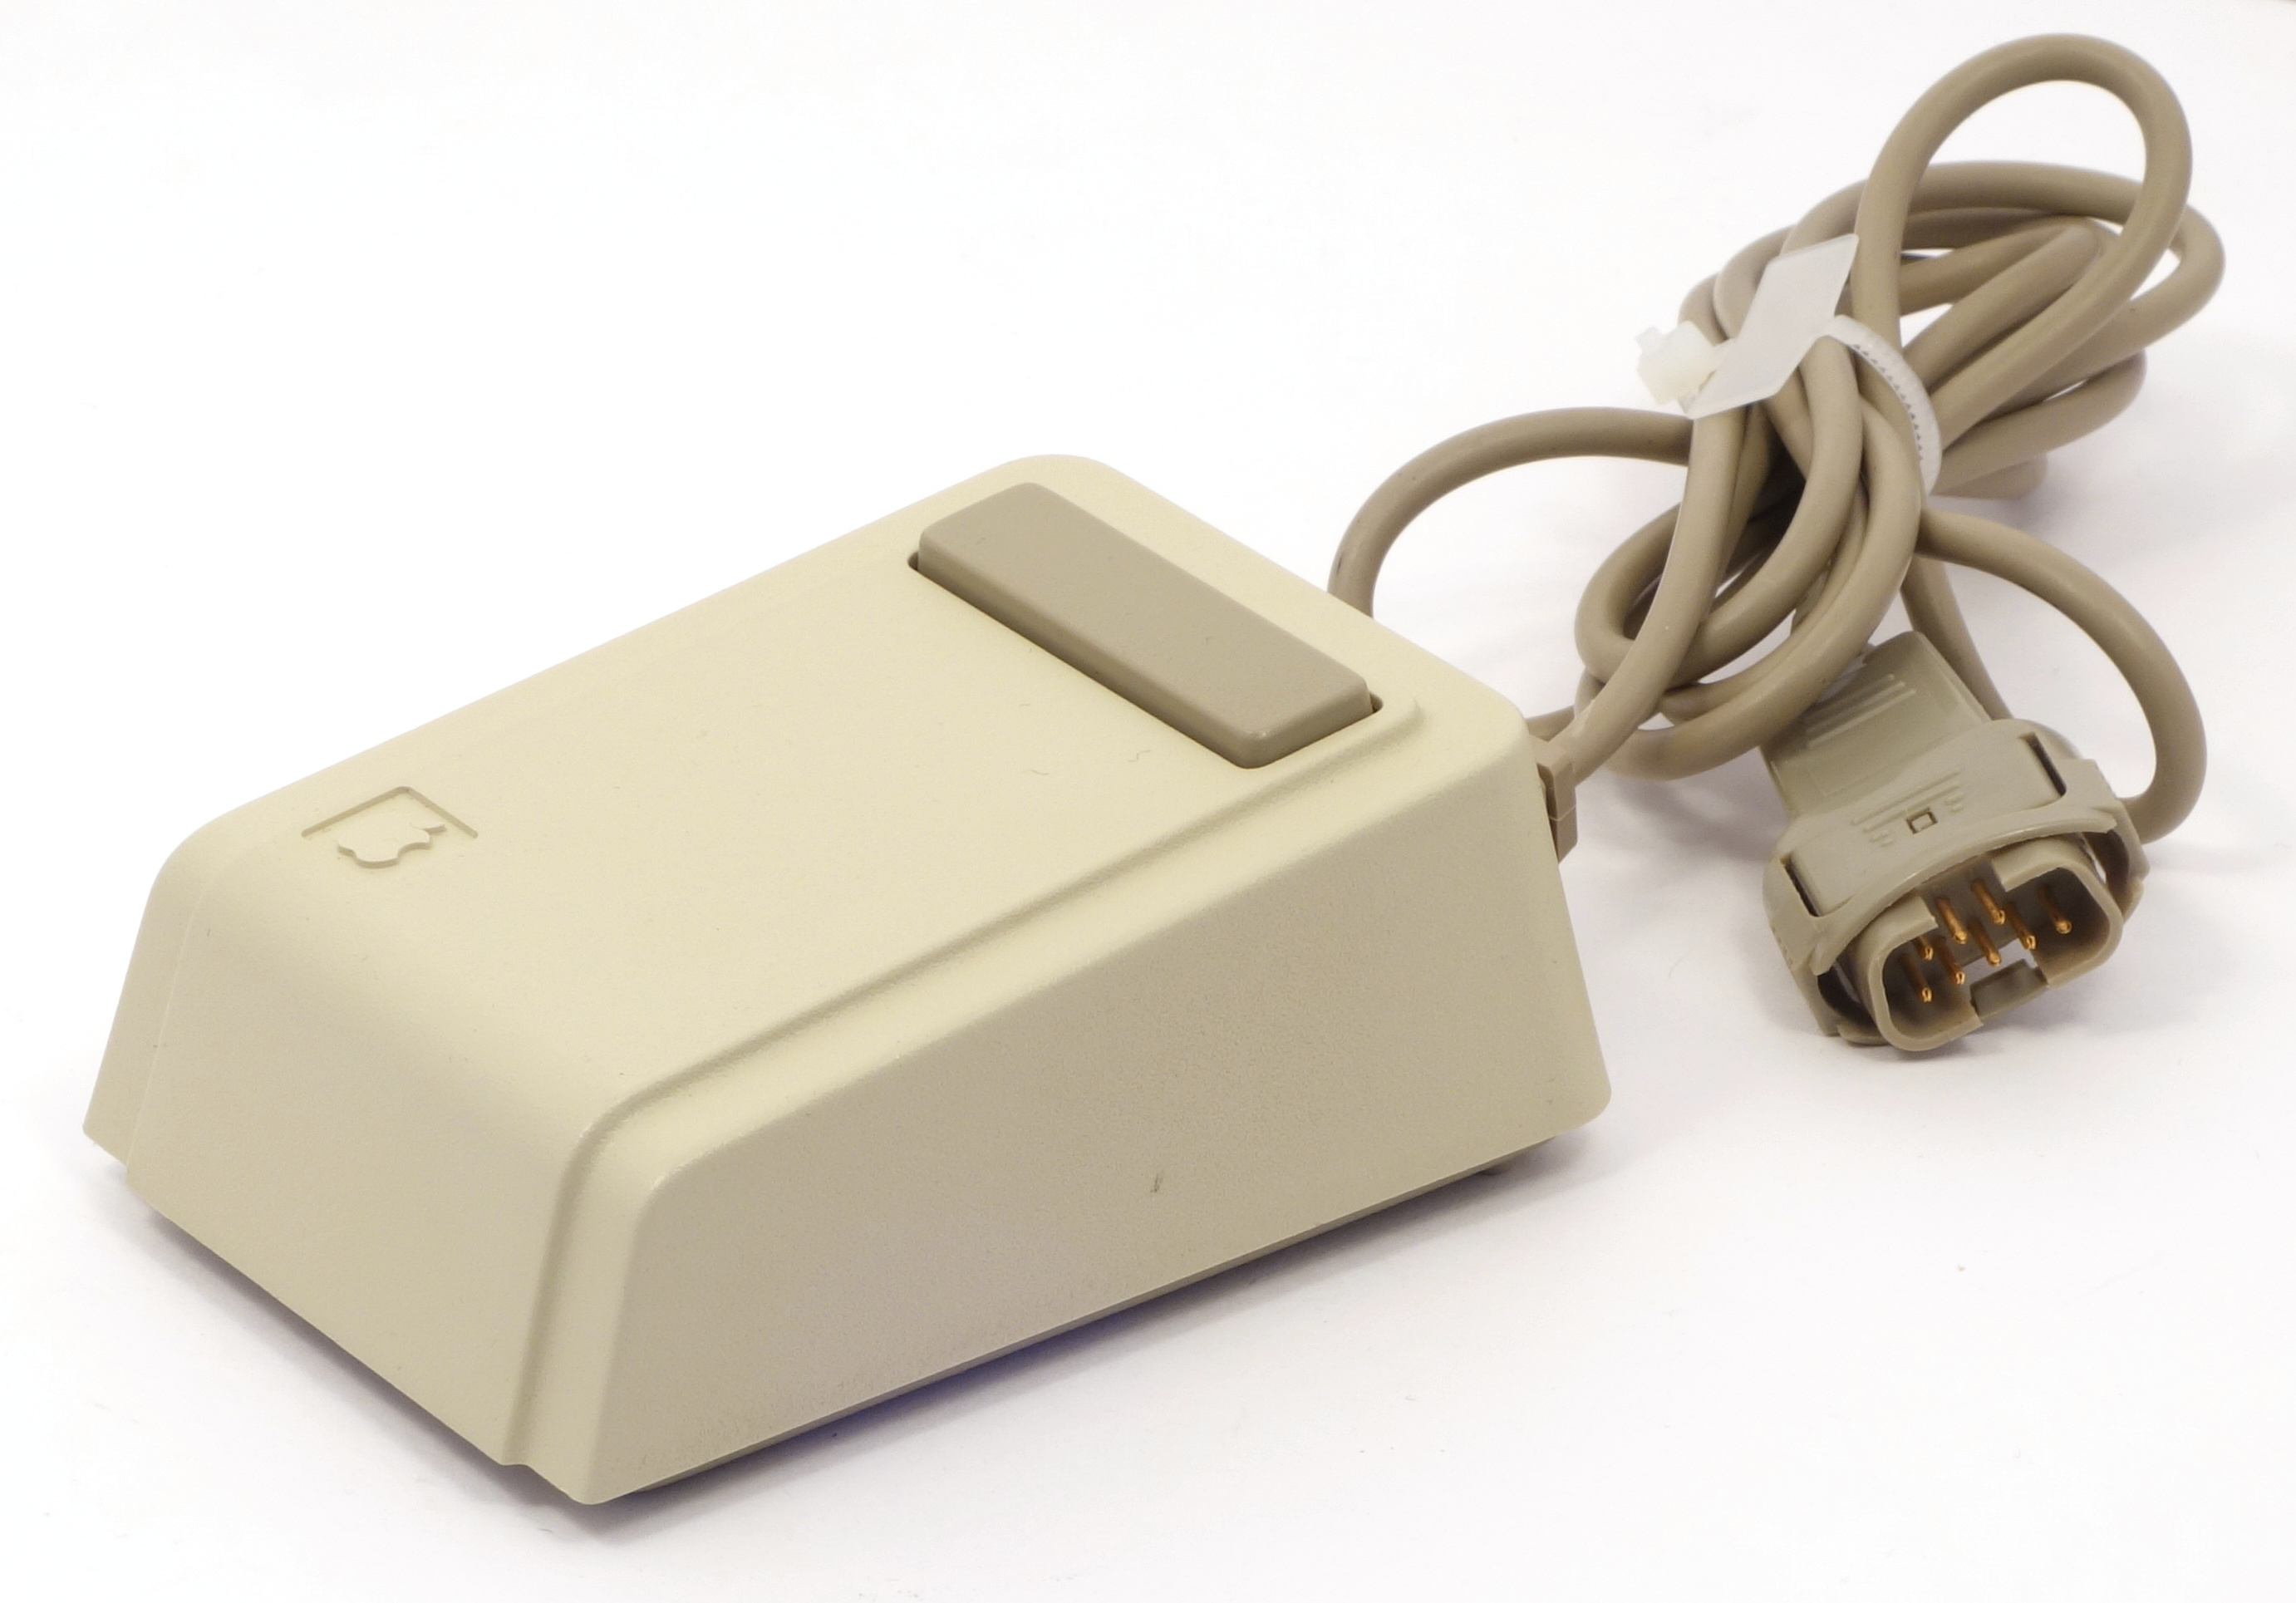
\includegraphics[scale=0.5]{1983_apple_lisa_mouse/applenorm_30.jpg}
    \caption{Apple Lisa mouse}
    \label{fig:AppleLisaPic}
\end{figure}

The mouse was manufactured by Apple, but the authorship of its development belongs to a third-party company, Hovey-Kelley (later renamed to IDEO). Based on the design of Xerox and Hawley Mouse House mice, the design team created a cheaper yet technically better mechanical part, and a complex internal structure of the case that holds the mouse parts together. Much attention was paid to other key components of the mouse, including the acoustic and tactile feel of the button and the rubberized coating on the ball \cite{ideo}.

\begin{figure}[h]
    \centering
    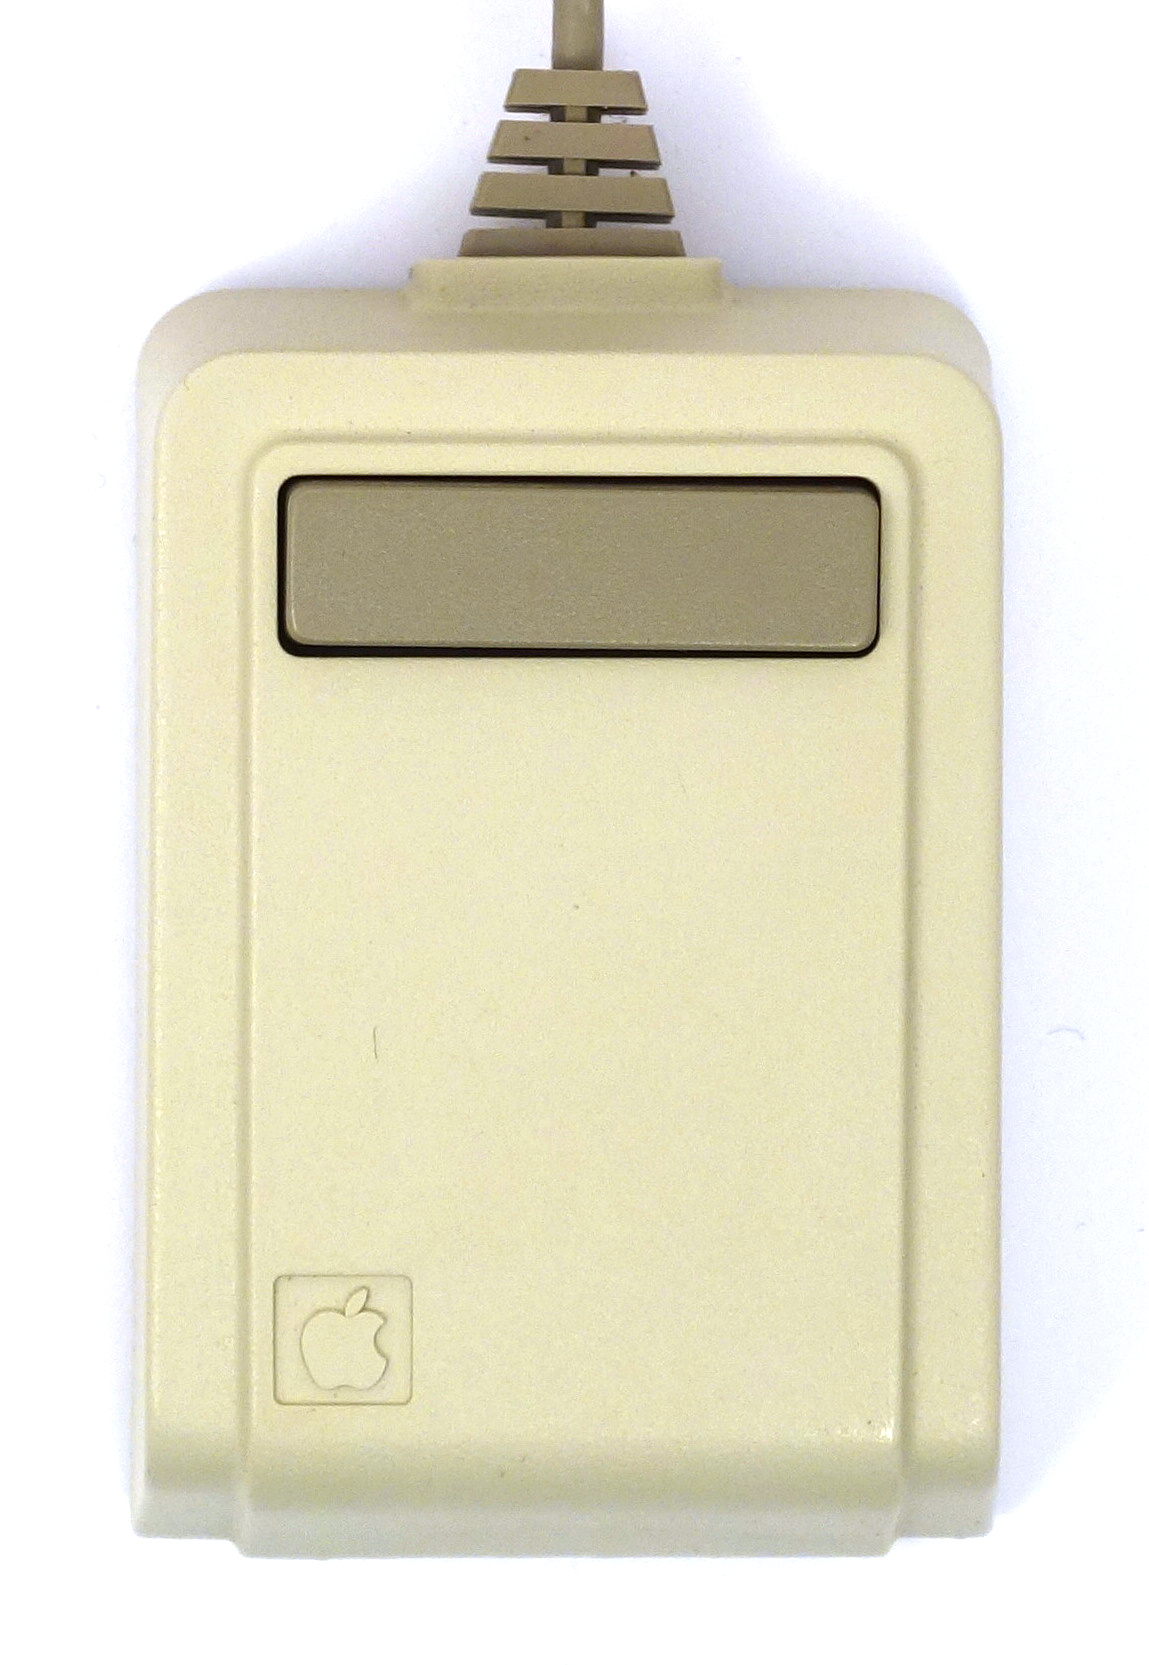
\includegraphics[scale=0.55]{1983_apple_lisa_mouse/appletop_60.jpg}
    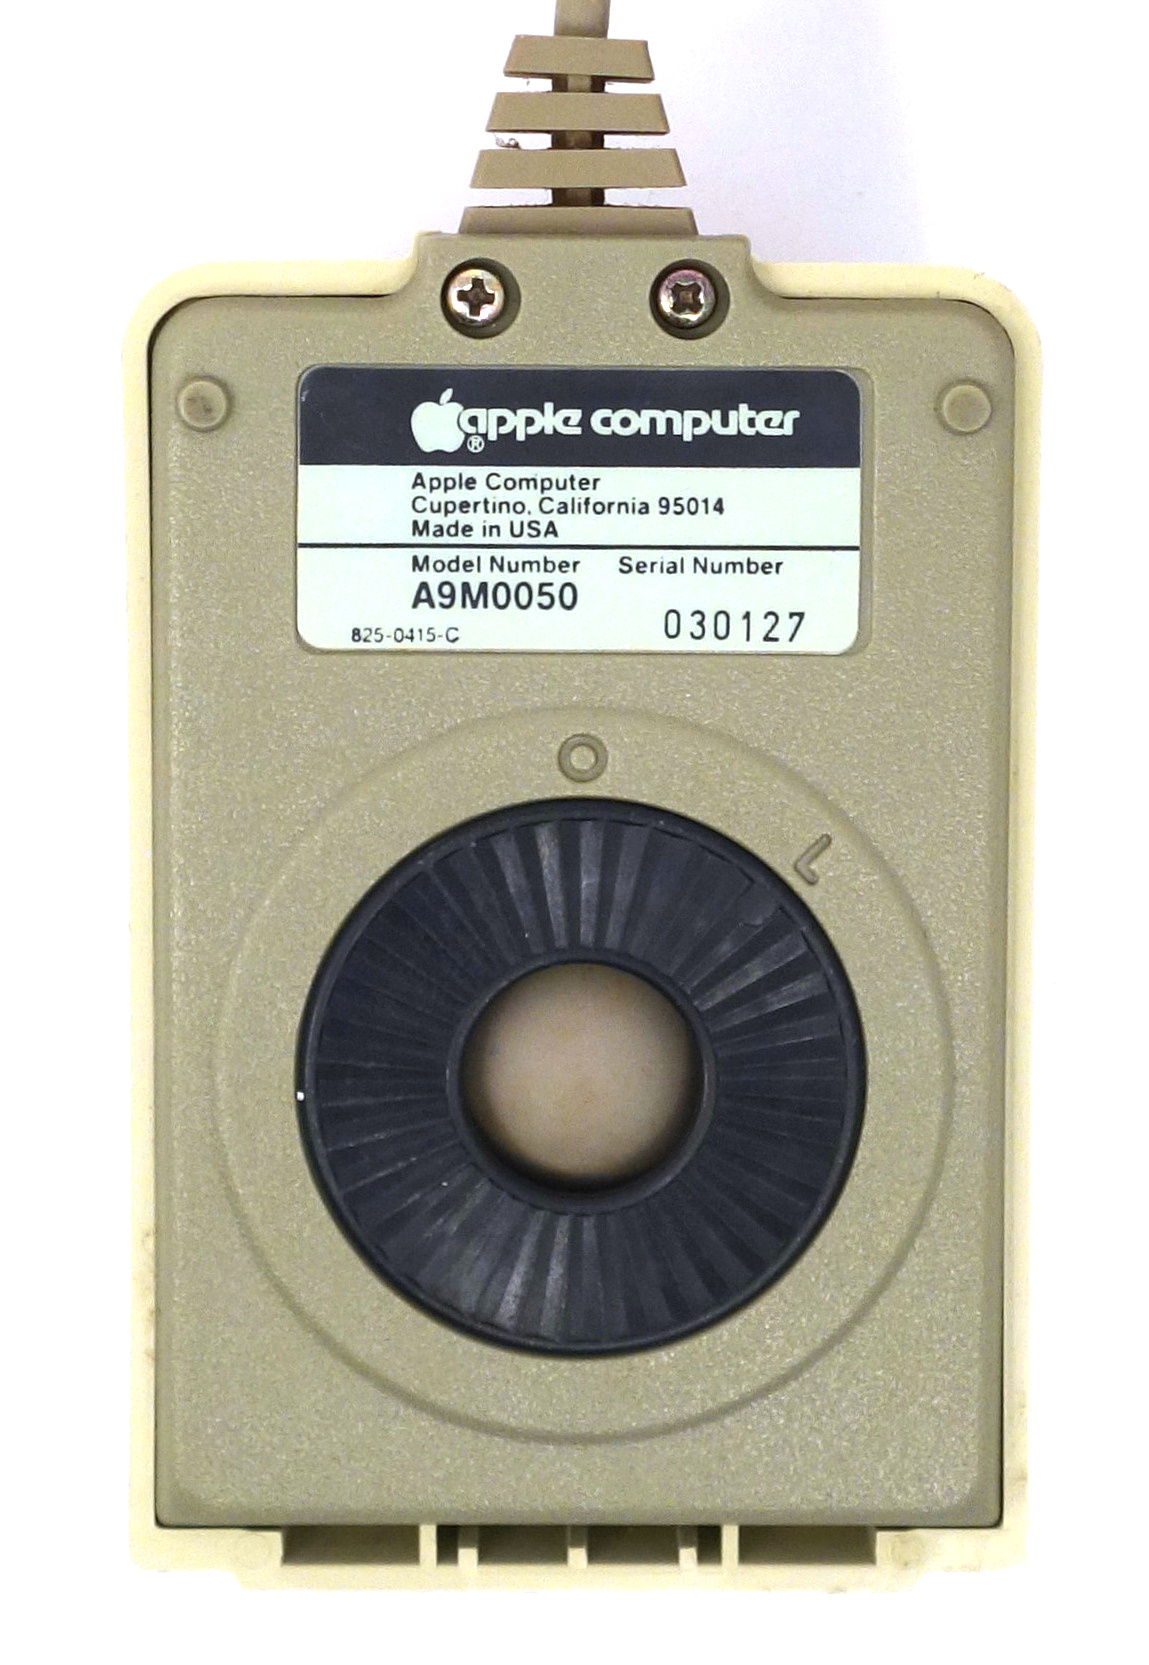
\includegraphics[scale=0.55]{1983_apple_lisa_mouse/applebottom_60.jpg}
    \caption{Apple Lisa mouse, top and bottom views}
    \label{fig:AppleLisaTopAndBottom}
\end{figure}

The body of the Lisa mouse is a beige slanted box. The underside of the mouse body, cable and button are brown. There is an embossed Apple logo on the case (figure \ref{fig:AppleLisaTopAndBottom}). The ball is made of metal and has a rubber coating for better grip, unlike earlier mice that had either a rubber or smooth steel ball. Later, a similar implementation of the ball will become the standard, as well as a removable ring that allows the user to easily remove the ball to clean the mouse from the collected debris, will become the standard. The same can be said about the basic design of its mechanism, which was later used in the vast majority of optomechanical mice.

\begin{figure}[h]
    \centering
    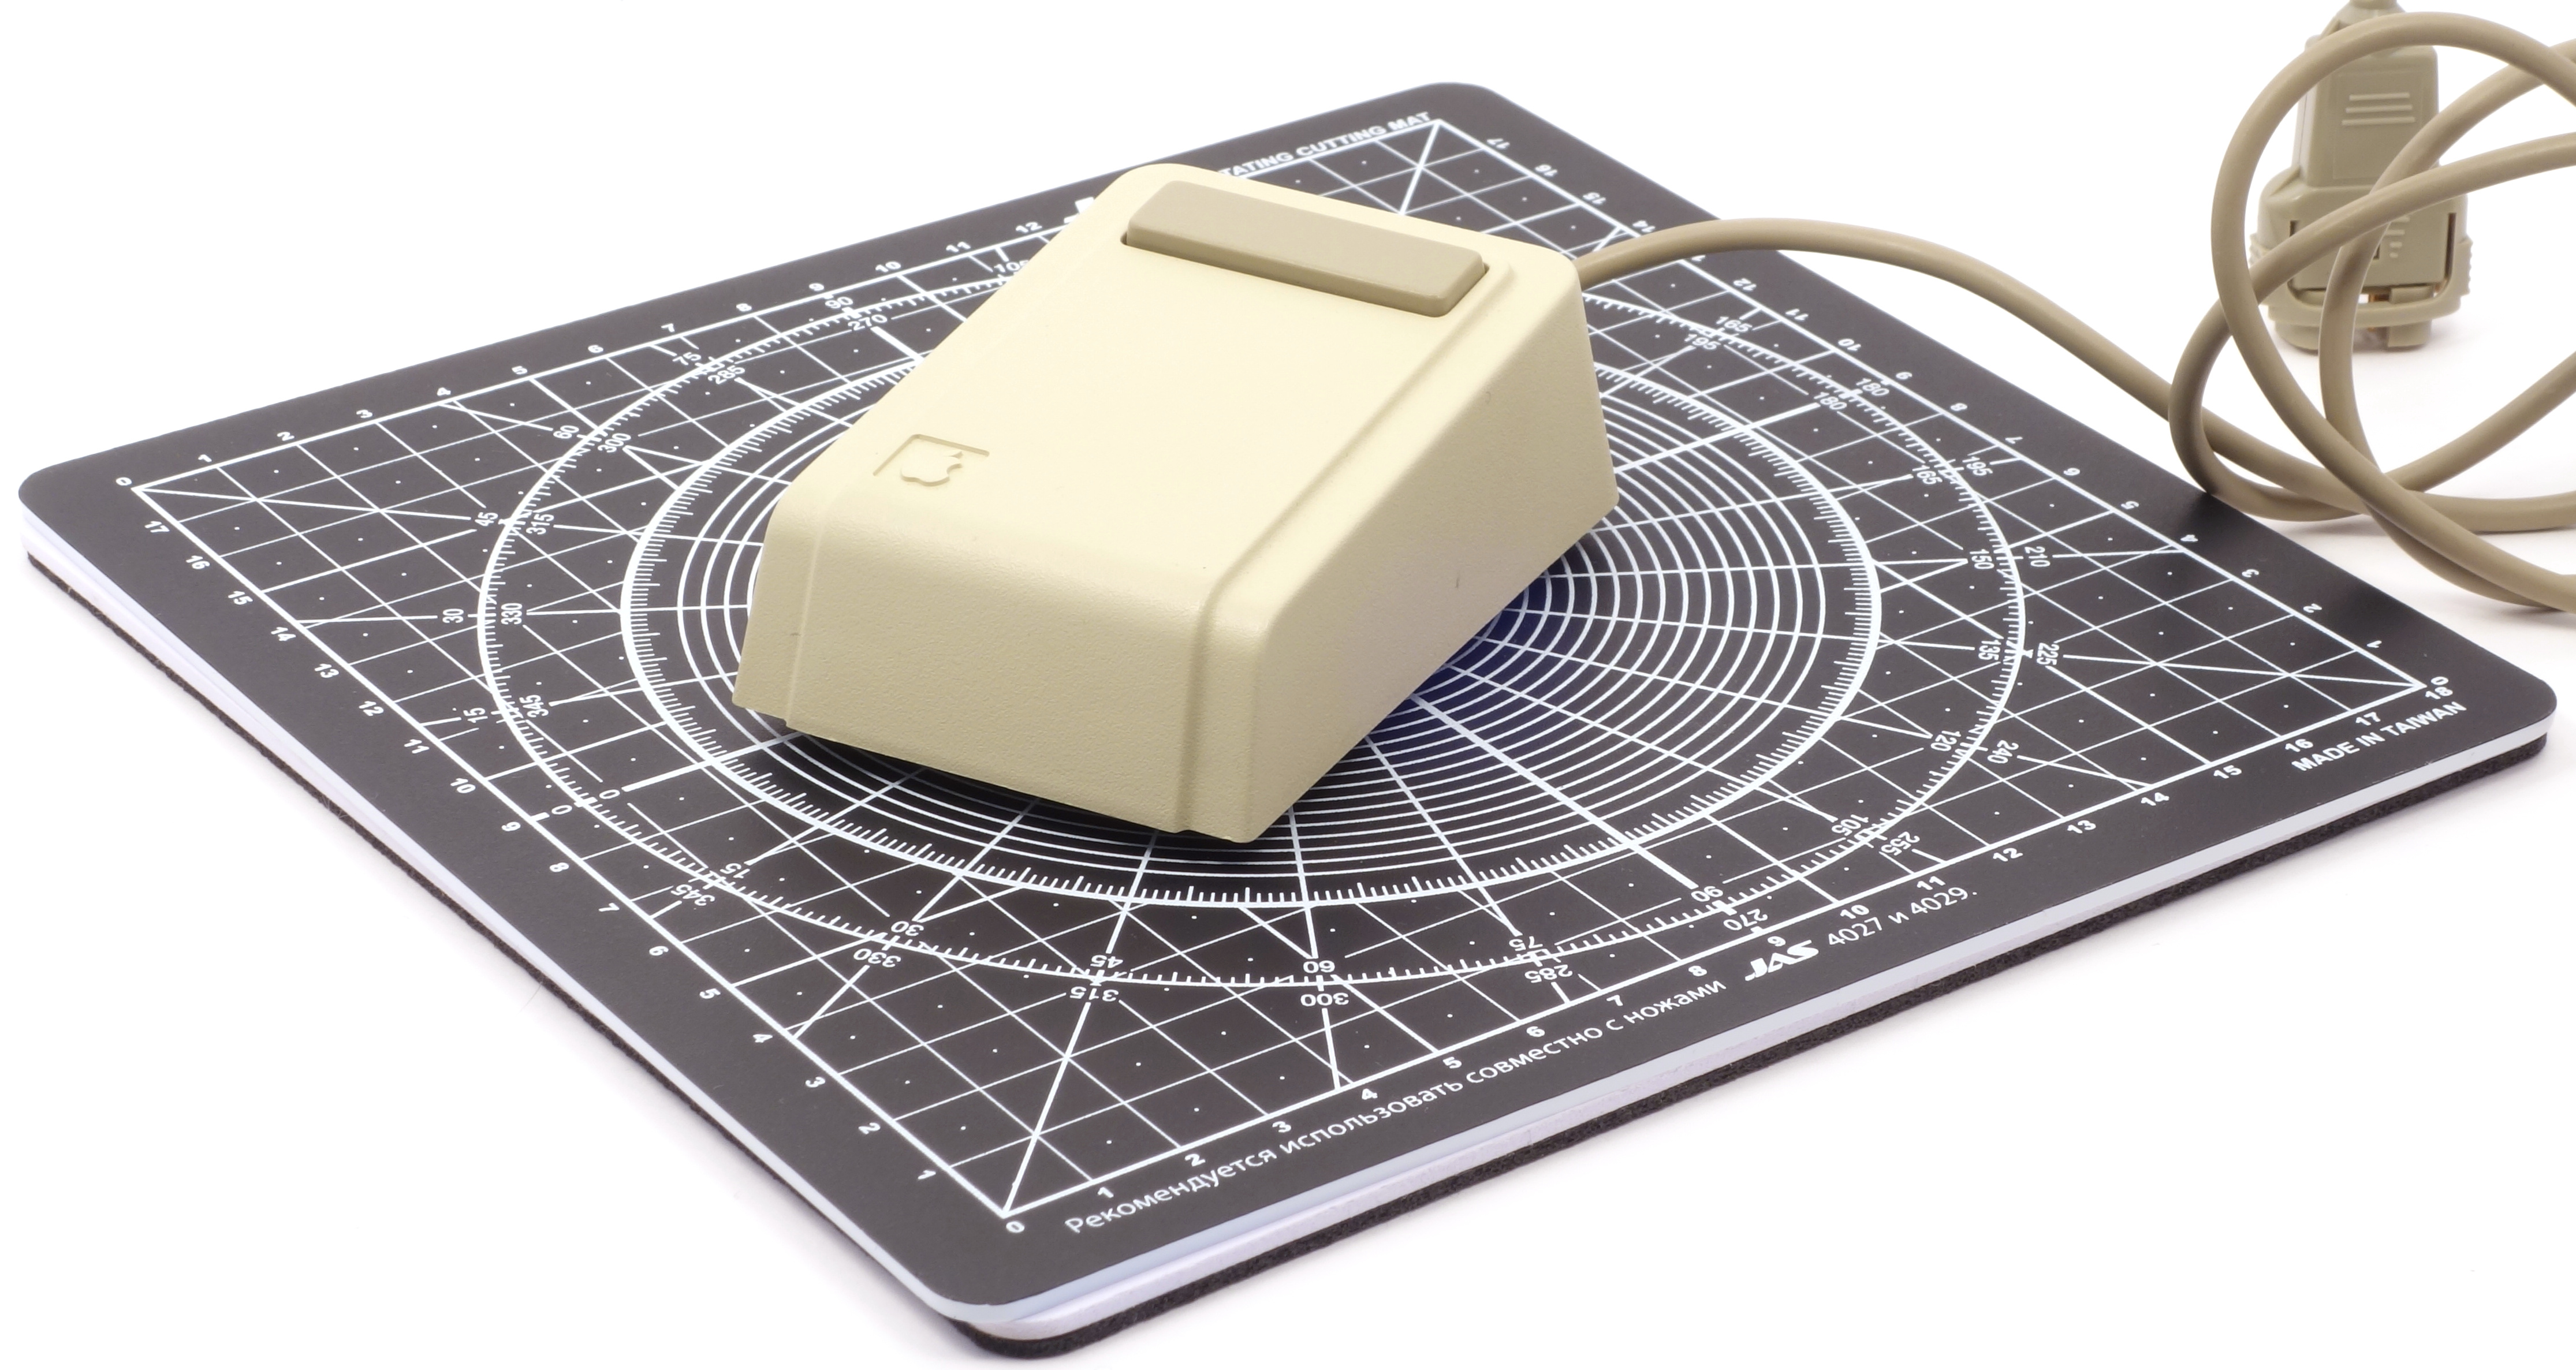
\includegraphics[scale=0.4]{1983_apple_lisa_mouse/applekovrik_60.jpg}
    \caption{Apple Lisa mouse on a graduated pad with a grid step of 1~cm}
    \label{fig:AppleLisaSize}
\end{figure}

Despite the relatively small size, however, typical of the mice of the 1980s (figure \ref{fig:AppleLisaSize}), the research of its developers has been useful, so it fits comfortably in the hand. At the same time, the only button is located orthogonally to the cable and is designed to be pressed with two fingers rather than one (figure \ref{fig:AppleLisaHand}), and the tactility of pressing is provided by a specially provided spring mechanism.

\begin{figure}[h]
    \centering
    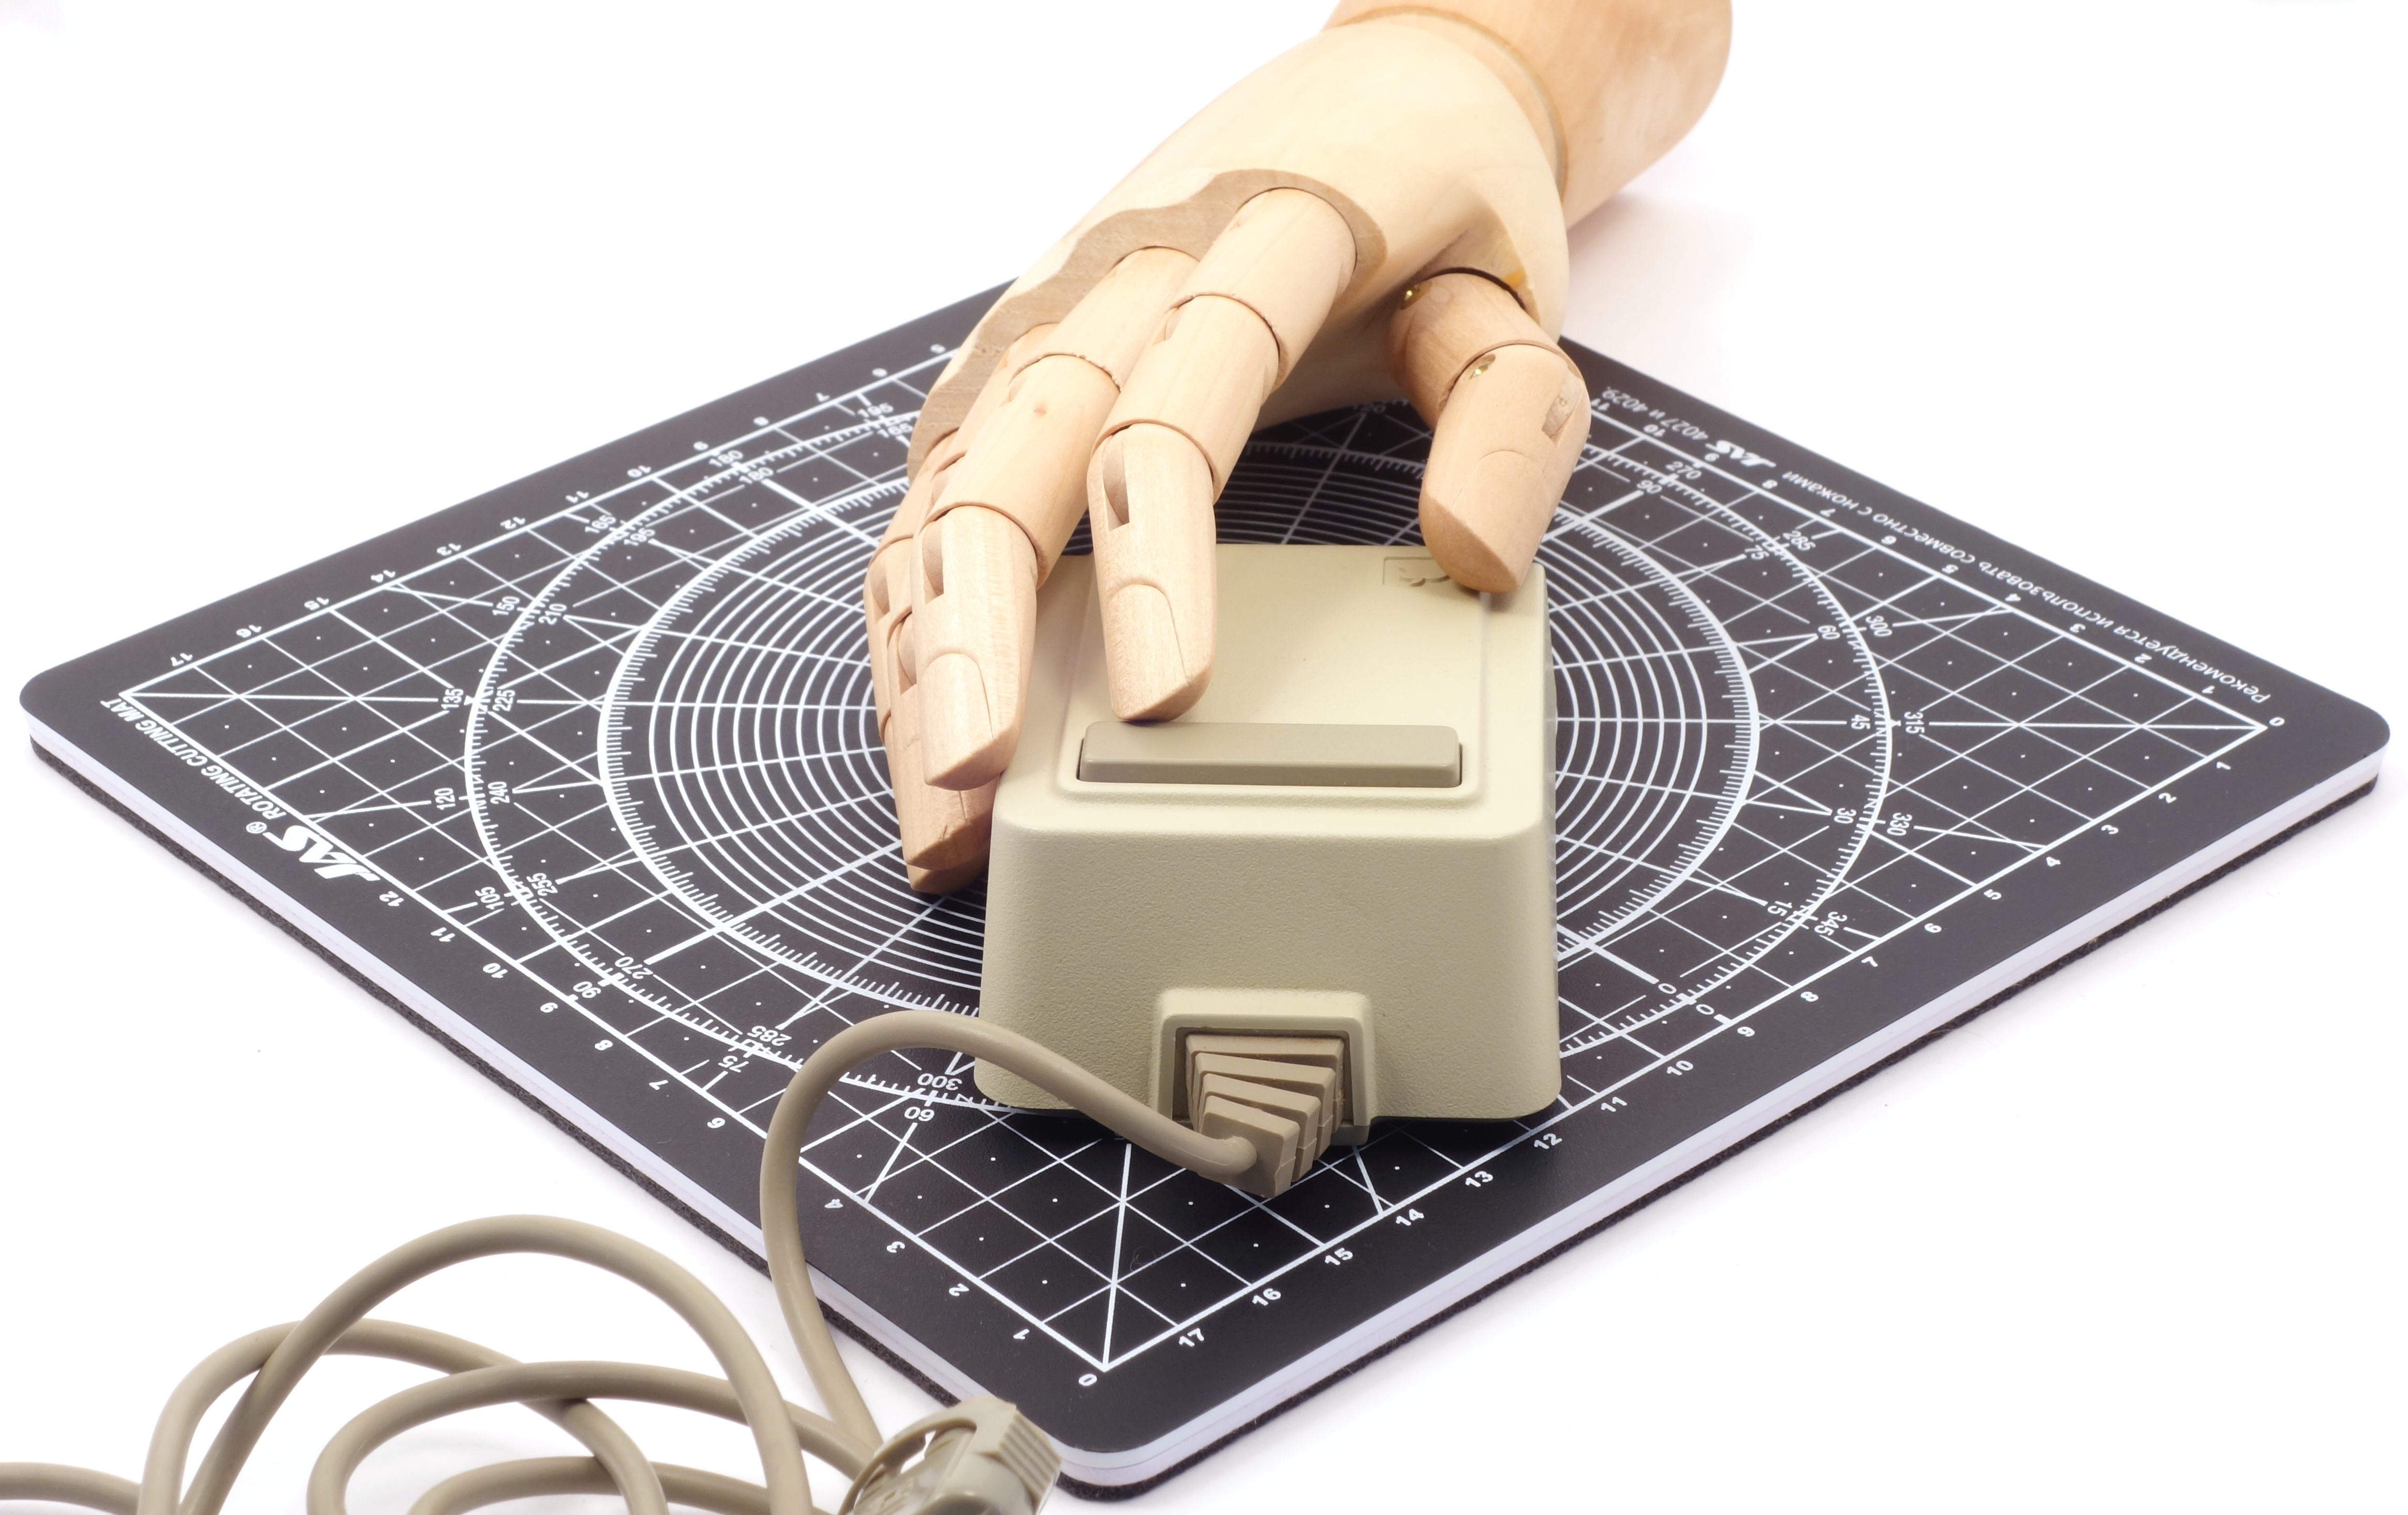
\includegraphics[scale=0.4]{1983_apple_lisa_mouse/appleruka_60.jpg}
    \caption{Apple Lisa mouse with a human hand model}
    \label{fig:AppleLisaHand}
\end{figure}

Mouse internals are shown on figure \ref{fig:AppleLisaInside}. A rather complex internal structure of the case with a significant number of partitions and additional supports can be noted. Having inherited the design of the optomechanical encoder practically unchanged, manufacturers of subsequent mice did step by step simplification of the case internal structure, reaching the almost hollow design of the device in the end of nineties.

 \begin{figure}[h]
    \centering
    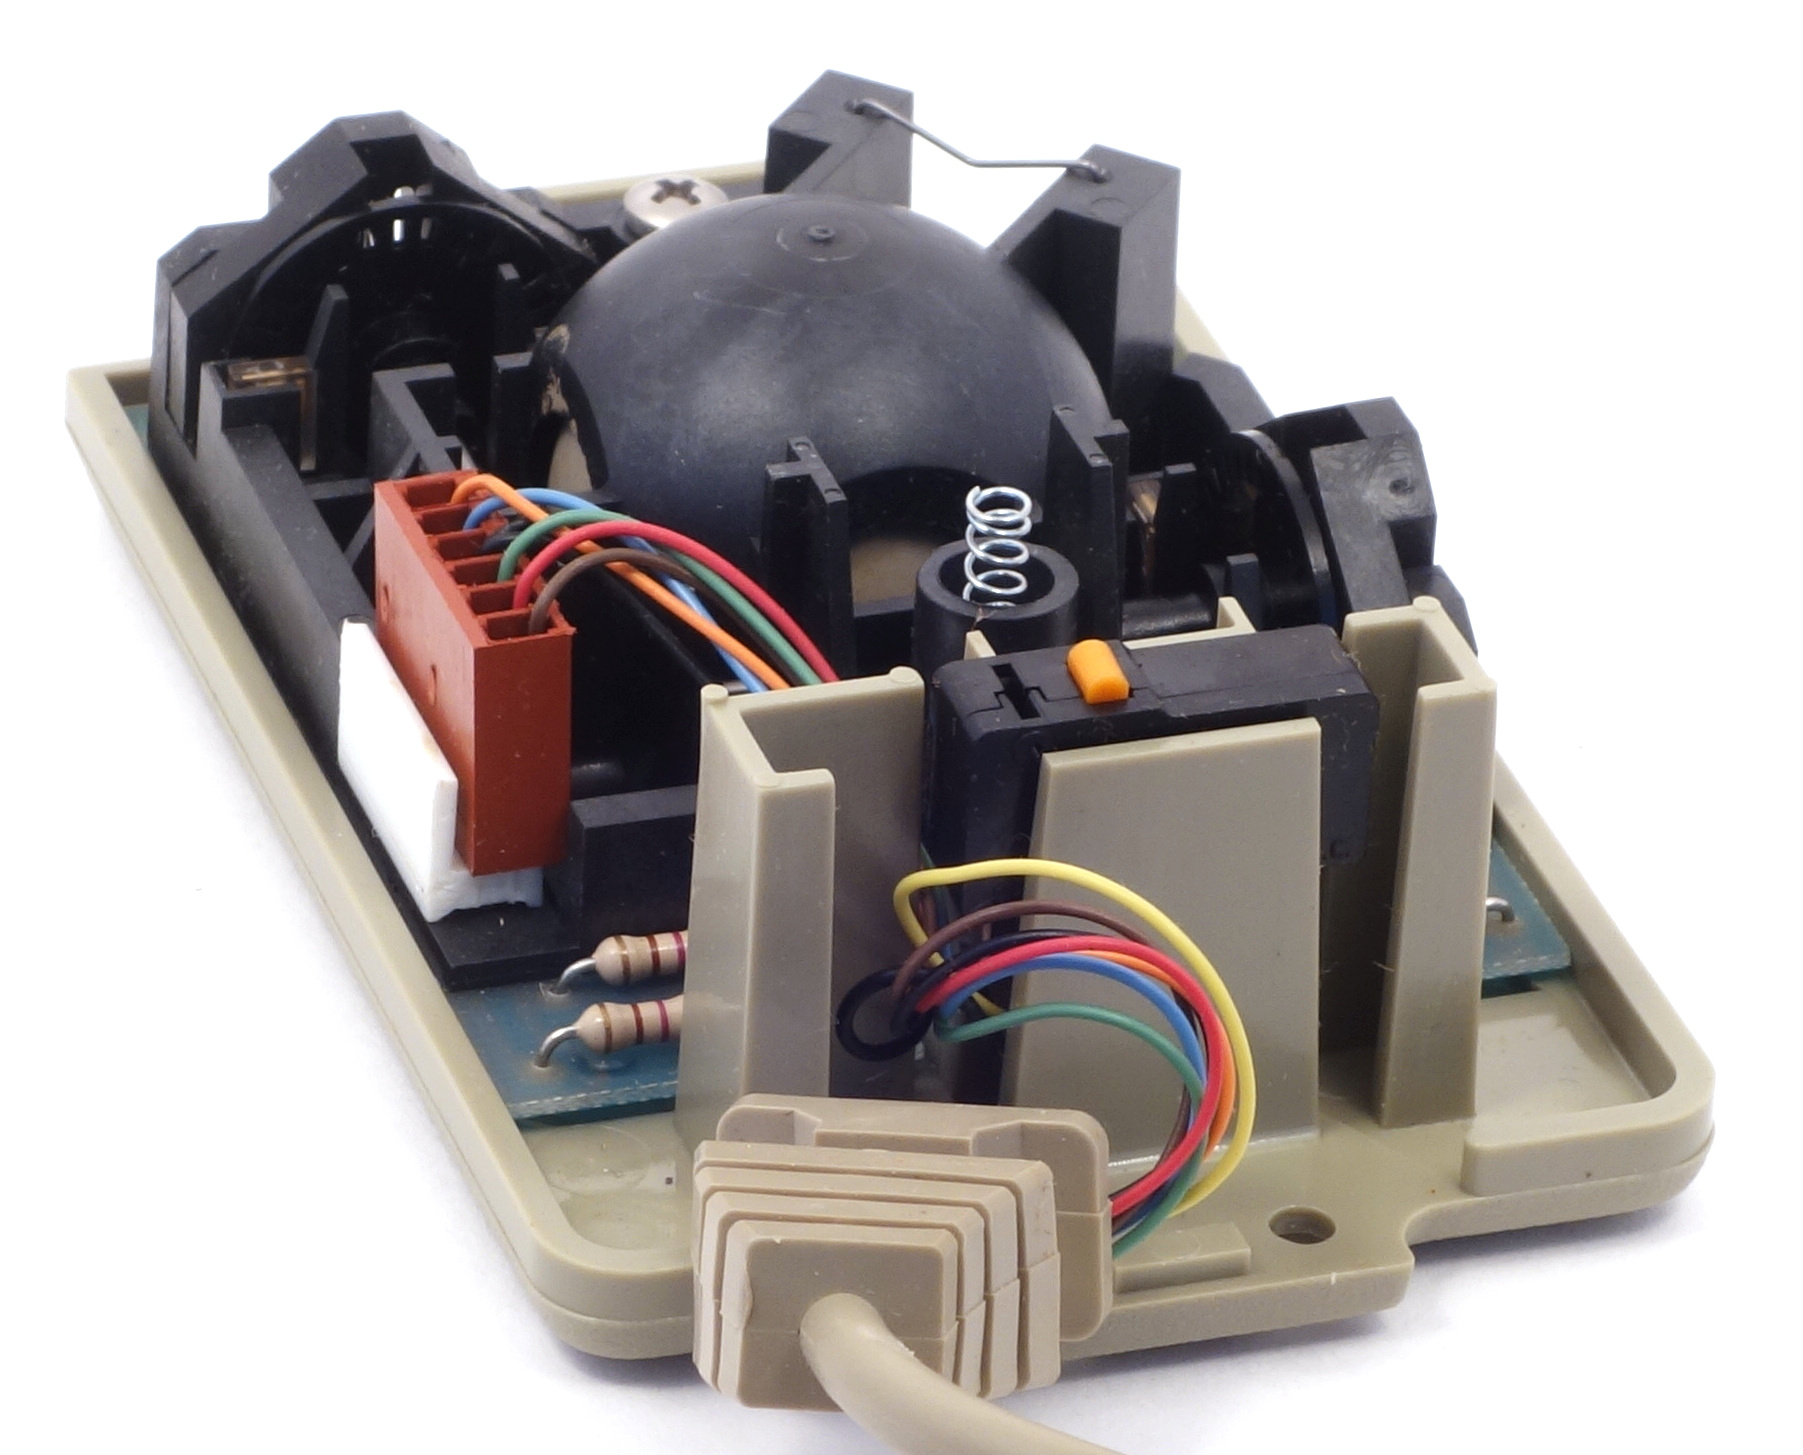
\includegraphics[scale=0.6]{1983_apple_lisa_mouse/appleraz_60.jpg}
    \caption{Apple Lisa mouse disassembled}
    \label{fig:AppleLisaInside}
\end{figure}

\begin{thebibliography}{9}
\bibitem {mouses} Apple Lisa I Mouse \url{https://www.oldmouse.com/mouse/apple/lisa.shtml}

\bibitem {ideo} Creating the First Usable Mouse \url{https://www.ideo.com/case-study/creating-the-first-usable-mouse}
\end{thebibliography}
\end{document}
